\documentclass[tikz,border=2pt]{standalone}
\usepackage{amsmath,amssymb}
\usepackage{pgfplots}
\pgfplotsset{compat=1.18}

\begin{document}
% Adam's law for X ~ Unif(0,1), Y | X ~ Bin(10, X): the conditional mean g(x) = 10x is averaged
% over X; the area under g (weights f_X = 1) is E[Y] = 5.
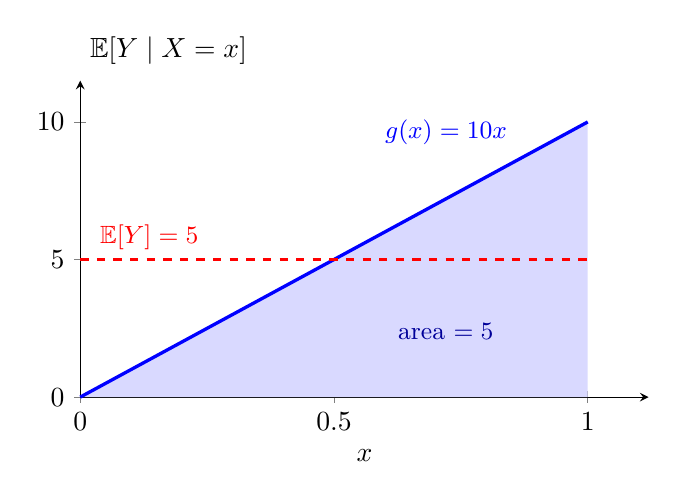
\begin{tikzpicture}
	\begin{axis}[
		axis lines=left, xmin=0, xmax=1.12, ymin=0, ymax=11.5,
		xtick={0,0.5,1}, ytick={0,5,10},
		xlabel={$x$}, ylabel={$\mathbb{E}[Y\mid X=x]$}, ylabel style={rotate=-90, anchor=south west, at={(axis description cs:0,1.02)}},
		width=8.8cm, height=5.6cm, clip=false
		]
		\addplot[fill=blue!15, draw=none, domain=0:1] {10*x} \closedcycle;
		\addplot[blue, very thick, domain=0:1] {10*x};
		\draw[red, dashed, thick] (axis cs:0,5) -- (axis cs:1,5);
		\node[red, anchor=south west, font=\small] at (axis cs:0.02,5) {$\mathbb{E}[Y]=5$};
		\node[blue, anchor=south east, font=\small] at (axis cs:0.86,8.8) {$g(x)=10x$};
		\node[blue!60!black, font=\small] at (axis cs:0.72,2.4) {area $=5$};
	\end{axis}
	
\end{tikzpicture}
\end{document}
